\chapter{कोशिका चक्र और समसूत्री विभाजन}\label{ch:g11:cell-cycle-mitosis}

प्याज़ की जड़ का सिरा किसी कवर स्लिप के नीचे कुचलिए, उसे रँगिए, और
देखिए: गोल \omterm{def:g10:cells-common-unit:organelle}{केंद्रक} वाली सैकड़ों शांत \omterm{def:g10:cells-common-unit:cell}{कोशिकाओं} के बीच कुछ \omterm{def:g10:cells-common-unit:cell}{कोशिकाएँ} कुछ और
ही दिखाती हैं --- \omterm{def:g10:cells-common-unit:cell}{कोशिका} के बीचोबीच जमा गहरे X जैसे छड़, या सिरों की ओर
खिंचे छड़ों के दो जत्थे, या दो छोटे \omterm{def:g10:cells-common-unit:organelle}{केंद्रक} जिनके बीच एक दीवार बन रही
है। आप \omterm{def:g10:cells-common-unit:cell}{कोशिका} विभाजन को अलग-अलग क्षणों पर पकड़े हुए देख रहे हैं, उस ऊतक
में जो रोज़ एक मिलीमीटर बढ़ता है। उन विभाजनों में से हर एक दो पुत्री
\omterm{def:g10:cells-common-unit:cell}{कोशिकाओं} को \omterm{def:g10:universal-dna:information}{गुणसूत्रों} के दो पूरे और एक जैसे जत्थे सौंप देता है। यह अध्याय
किसी \omterm{def:g10:cells-common-unit:cell}{कोशिका} का एक पूरे चक्र भर पीछा करता है, और उस घंटे को क़रीब से देखता
है जिसमें \omterm{def:g11:cell-cycle-mitosis:chromosome}{गुणसूत्र} बाँटे जाते हैं।

\section{कोशिका चक्र}

\begin{definition}[कोशिका चक्र]\label{def:g11:cell-cycle-mitosis:cycle}
\emph{कोशिका चक्र}\index{कोशिका चक्र} किसी \omterm{def:g10:cells-common-unit:cell}{कोशिका} के विभाजन से जन्म लेने
से लेकर उसके ख़ुद दो में बँटने तक की घटनाओं का क्रम है। उसमें
\emph{अंतरावस्था} है, जिसके दौरान \omterm{def:g10:cells-common-unit:cell}{कोशिका} बढ़ती है और अपना \omterm{def:g10:universal-dna:information}{DNA} नक़ल करती
है, और \emph{M प्रावस्था}, जिसके दौरान पहले \omterm{def:g10:cells-common-unit:organelle}{केंद्रक} बँटता है
(\emph{समसूत्री विभाजन}\index{समसूत्री विभाजन}) और फिर \omterm{def:g10:cells-common-unit:cell}{कोशिकाद्रव्य}
(\emph{\omterm{def:g10:cells-common-unit:cell}{कोशिकाद्रव्य} विभाजन})। अंतरावस्था के तीन हिस्से हैं:
$\mathrm{G_1}$ (वृद्धि), S (\omterm{def:g11:dna-replication:replication}{DNA का प्रतिकृतिकरण},
\cref{ch:g11:dna-replication}) और $\mathrm{G_2}$ (विभाजन की तैयारी)।
\end{definition}

\begin{omfigure}
\begin{tikzpicture}[font=\small]
  % pie: G1 11h, S 8h, G2 4h, M 1h  (24h) -> angles: G1 165°, S 120°, G2 60°, M 15°
  \fill[omDef!30] (0,0) -- (90:2.2) arc (90:-75:2.2) -- cycle;
  \fill[omProp!35] (0,0) -- (-75:2.2) arc (-75:-195:2.2) -- cycle;
  \fill[omMeth!35] (0,0) -- (-195:2.2) arc (-195:-255:2.2) -- cycle;
  \fill[omThm!50] (0,0) -- (-255:2.2) arc (-255:-270:2.2) -- cycle;
  \draw[thick] (0,0) circle (2.2);
  \foreach \a in {90,-75,-195,-255} \draw[thick] (0,0) -- (\a:2.2);
  \node at (10:1.3) {$\mathrm{G_1}$};
  \node at (-135:1.3) {S};
  \node at (-225:1.35) {$\mathrm{G_2}$};
  \node[anchor=south east] at (-262:2.35) {M};
  \node[anchor=west, align=left] at (2.6,1.3) {$\mathrm{G_1}$: वृद्धि, लगभग \qty{11}{h}};
  \node[anchor=west, align=left] at (2.6,0.5) {S: DNA का प्रतिकृतिकरण, \qty{8}{h}};
  \node[anchor=west, align=left] at (2.6,-0.3) {$\mathrm{G_2}$: तैयारी, \qty{4}{h}};
  \node[anchor=west, align=left] at (2.6,-1.1) {M: समसूत्री और कोशिकाद्रव्य विभाजन, \qty{1}{h}};
  \draw[->, thick] (100:2.5) arc (100:130:2.5);
\end{tikzpicture}

{\small किसी ठेठ विभाजित होती मानव \omterm{def:g10:cells-common-unit:cell}{कोशिका} का \omterm{def:g11:cell-cycle-mitosis:cycle}{कोशिका चक्र}, लगभग 24 घंटे
का। अंतरावस्था ($\mathrm{G_1}$, S, $\mathrm{G_2}$) उनमें से 23 ले लेती
है; और ख़ुद विभाजन एक। बहुत-सी \omterm{def:g10:cells-common-unit:cell}{कोशिकाएँ} $\mathrm{G_1}$ के बाद चक्र छोड़
देती हैं और फिर कभी विभाजित नहीं होतीं।}
\end{omfigure}

\begin{proposition}[चक्र भर में DNA]\label{prop:g11:cell-cycle-mitosis:dna}
विभाजन के ठीक बाद \omterm{def:g10:cells-common-unit:organelle}{केंद्रक} में \omterm{def:g10:universal-dna:information}{DNA} की मात्रा को $q$ कहिए। वह $q$ पर पूरे
$\mathrm{G_1}$ भर टिकी रहती है, S के दौरान \omterm{def:g10:universal-dna:information}{गुणसूत्रों} की नक़ल बनने के
साथ लगातार बढ़कर $2q$ हो जाती है, फिर $2q$ पर ही पूरे $\mathrm{G_2}$ और
\omterm{def:g11:cell-cycle-mitosis:cycle}{समसूत्री विभाजन} के पहले हिस्से भर बनी रहती है, और उसके अंत में हर
पुत्री \omterm{def:g10:cells-common-unit:organelle}{केंद्रक} में गिरकर फिर $q$ रह जाती है। S के दौरान \omterm{def:g10:universal-dna:information}{गुणसूत्रों} की
संख्या नहीं बदलती: हर \omterm{def:g11:cell-cycle-mitosis:chromosome}{गुणसूत्र} की नक़ल दो एक जैसे \emph{\omterm{def:g11:cell-cycle-mitosis:chromosome}{क्रोमैटिडों}} में
होती है, जो अपने \emph{\omterm{def:g11:cell-cycle-mitosis:chromosome}{सेंट्रोमियर}} पर आपस में जुड़े रहते हैं, और वे
\omterm{def:g11:cell-cycle-mitosis:cycle}{समसूत्री विभाजन} के दौरान ही दो \omterm{def:g10:universal-dna:information}{गुणसूत्रों} में अलग होते हैं।
\end{proposition}
\admitted

\begin{omfigure}
\begin{tikzpicture}
\begin{axis}[
  width=0.9\linewidth, height=5.4cm,
  axis x line=bottom, axis y line=left,
  xmin=0, xmax=50, ymin=0, ymax=2.8,
  xlabel={समय (\unit{h})}, ylabel={प्रति केंद्रक DNA},
  xlabel style={font=\small, at={(axis description cs:0.5,-0.1)}, anchor=north},
  ylabel style={font=\small},
  tick label style={font=\small}, xtick={0,11,19,23,24,35,43,47,48},
  xticklabels={0,11,19,23,,24,35,43,,48},
  ytick={1,2}, yticklabels={$q$, $2q$},
  clip=false,
]
\addplot[thick, omDef] coordinates {(0,1) (11,1) (19,2) (23,2) (23.9,2) (24,1) (35,1) (43,2) (47,2) (47.9,2) (48,1) (50,1)};
\node[font=\small, anchor=south] at (axis cs:5.5,2.25) {$\mathrm{G_1}$};
\node[font=\small, anchor=south] at (axis cs:15,2.25) {S};
\node[font=\small, anchor=south] at (axis cs:21,2.25) {$\mathrm{G_2}$};
\node[font=\small, anchor=south] at (axis cs:29.5,2.25) {$\mathrm{G_1}$};
\node[font=\small, anchor=south] at (axis cs:39,2.25) {S};
\node[font=\small, anchor=south] at (axis cs:45,2.25) {$\mathrm{G_2}$};
\node[font=\small, anchor=south, omThm] at (axis cs:23.5,2.55) {M};
\node[font=\small, anchor=south, omThm] at (axis cs:47.5,2.55) {M};
\draw[dashed, gray] (axis cs:11,0) -- (axis cs:11,2.2);
\draw[dashed, gray] (axis cs:19,0) -- (axis cs:19,2.2);
\draw[dashed, gray] (axis cs:23,0) -- (axis cs:23,2.2);
\draw[dashed, gray] (axis cs:24,0) -- (axis cs:24,2.2);
\draw[dashed, gray] (axis cs:35,0) -- (axis cs:35,2.2);
\draw[dashed, gray] (axis cs:43,0) -- (axis cs:43,2.2);
\draw[dashed, gray] (axis cs:47,0) -- (axis cs:47,2.2);
\end{axis}
\end{tikzpicture}

{\small 24 घंटे के दो लगातार चक्रों पर किसी एक \omterm{def:g10:cells-common-unit:organelle}{केंद्रक} में \omterm{def:g10:universal-dna:information}{DNA} की मात्रा।
वह S के दौरान दोगुनी होती है और \omterm{def:g11:cell-cycle-mitosis:cycle}{समसूत्री विभाजन} के अंत में आधी; और पुत्री
\omterm{def:g10:cells-common-unit:cell}{कोशिका} हमेशा $q$ से शुरू करती है।}
\end{omfigure}

\begin{example}[वक्र पढ़ना]\label{ex:g11:cell-cycle-mitosis:reading}
$2q$ पर नापी गई \omterm{def:g10:cells-common-unit:cell}{कोशिका} $\mathrm{G_2}$ में हो सकती है या शुरुआती \omterm{def:g11:cell-cycle-mitosis:cycle}{समसूत्री
विभाजन} में; $1.5q$ पर वह पक्के तौर पर S में है, यानी प्रतिकृतिकरण के
बीचोबीच; और $q$ पर वह $\mathrm{G_1}$ में है --- या फिर उसने चक्र हमेशा के
लिए छोड़ दिया है, जैसे कोई न्यूरॉन या \omterm{def:g10:muscles-and-joints:muscle}{पेशी तंतु}, जो जीवन भर $q$ पर बने
रहते हैं। जिस ऊतक की हर \omterm{def:g10:cells-common-unit:cell}{कोशिका} $q$ पर हो, वह ऊतक विभाजित होना बंद कर चुका
है।
\end{example}

\section{गुणसूत्र, देखे हुए}

\begin{definition}[गुणसूत्र, क्रोमैटिड, गुणसूत्र-चित्र]\label{def:g11:cell-cycle-mitosis:chromosome}
\emph{गुणसूत्र} अपने कसने वाले प्रोटीनों समेत एक \omterm{def:g10:universal-dna:information}{DNA} अणु है। विभाजनों के
बीच वह एक ढीला, अदृश्य धागा होता है; और \omterm{def:g11:cell-cycle-mitosis:cycle}{समसूत्री विभाजन} के शुरू में वह
कुंडलित होकर प्रकाश सूक्ष्मदर्शी से दिखने वाली सघन छड़ बन जाता है।
प्रतिकृतिकरण के बाद हर गुणसूत्र दो एक जैसे
\emph{क्रोमैटिडों}\index{क्रोमैटिड} से बना होता है, जो
\emph{सेंट्रोमियर}\index{सेंट्रोमियर} पर जुड़े रहते हैं: यानी वही जाना-पहचाना
X आकार। किसी \omterm{def:g10:biodiversity-scales:species}{जाति} का \emph{गुणसूत्र-चित्र}\index{गुणसूत्र-चित्र} उसके
\omterm{def:g10:universal-dna:information}{गुणसूत्रों} का पूरा जत्था है, जिसकी तस्वीर मध्यावस्था में ली जाती है और जिसे
आकार के हिसाब से जोड़ों में सजाया जाता है: मानव \omterm{def:g10:cells-common-unit:cell}{कोशिका} में 46 गुणसूत्र
होते हैं, 23 जोड़ों में, और किसी जोड़े के दोनों सदस्य \emph{\omterm{def:g10:common-ancestry:homology}{समजात}} होते
हैं --- यानी उन्हीं स्थानों पर वही \omterm{def:g10:universal-dna:gene}{जीन}, एक-एक हर जनक से।
\end{definition}

\begin{omfigure}
\begin{tikzpicture}[font=\scriptsize, line cap=round]
  % 22 autosome pairs of decreasing size, then X and Y; each chromosome = two chromatids
  \tikzset{chrom/.style={line width=2.6pt, omDef!75}}
  \foreach \n/\h/\c in {1/2.4/0.55, 2/2.3/0.5, 3/2.0/0.5, 4/1.9/0.35, 5/1.8/0.35, 6/1.7/0.45, 7/1.55/0.42, 8/1.45/0.4}
    { \pgfmathsetmacro{\x}{(\n-1)*1.55}
      \draw[chrom] (\x,0) -- (\x,\h); \draw[chrom] (\x+0.22,0) -- (\x+0.22,\h);
      \fill[omThm] (\x+0.11,{\h*\c}) circle (2pt);
      \node[anchor=north] at (\x+0.11,-0.08) {\n}; }
  \foreach \n/\h/\c in {9/1.4/0.35, 10/1.35/0.35, 11/1.35/0.4, 12/1.3/0.3, 13/1.1/0.15, 14/1.05/0.15, 15/1.0/0.15, 16/0.9/0.45}
    { \pgfmathsetmacro{\x}{(\n-9)*1.55}
      \draw[chrom] (\x,-3.2) -- (\x,-3.2+\h); \draw[chrom] (\x+0.22,-3.2) -- (\x+0.22,-3.2+\h);
      \fill[omThm] (\x+0.11,{-3.2+\h*\c}) circle (2pt);
      \node[anchor=north] at (\x+0.11,-3.28) {\n}; }
  \foreach \n/\h/\c in {17/0.85/0.3, 18/0.8/0.2, 19/0.65/0.5, 20/0.65/0.5, 21/0.5/0.2, 22/0.5/0.2}
    { \pgfmathsetmacro{\x}{(\n-17)*1.55}
      \draw[chrom] (\x,-5.6) -- (\x,-5.6+\h); \draw[chrom] (\x+0.22,-5.6) -- (\x+0.22,-5.6+\h);
      \fill[omThm] (\x+0.11,{-5.6+\h*\c}) circle (2pt);
      \node[anchor=north] at (\x+0.11,-5.68) {\n}; }
  % sex chromosomes
  \draw[chrom] (9.3,-5.6) -- (9.3,-4.1); \draw[chrom] (9.52,-5.6) -- (9.52,-4.1); \fill[omThm] (9.41,-4.85) circle (2pt);
  \node[anchor=north] at (9.41,-5.68) {X};
  \draw[chrom] (10.85,-5.6) -- (10.85,-5.1); \draw[chrom] (11.07,-5.6) -- (11.07,-5.1); \fill[omThm] (10.96,-5.5) circle (2pt);
  \node[anchor=north] at (10.96,-5.68) {Y};
\end{tikzpicture}

{\small मानव \omterm{def:g11:cell-cycle-mitosis:chromosome}{गुणसूत्र-चित्र}, आरेख के रूप में: घटते आकार के हिसाब से गिने
गए साधारण \omterm{def:g10:universal-dna:information}{गुणसूत्रों} के 22 जोड़े, और फिर लिंग \omterm{def:g11:cell-cycle-mitosis:chromosome}{गुणसूत्र} --- यहाँ X और Y,
यानी कोई पुरुष। हर \omterm{def:g11:cell-cycle-mitosis:chromosome}{गुणसूत्र} अपने दोनों \omterm{def:g11:cell-cycle-mitosis:chromosome}{क्रोमैटिडों} के रूप में खींचा गया
है, और \omterm{def:g11:cell-cycle-mitosis:chromosome}{सेंट्रोमियर} लाल है।}
\end{omfigure}

\begin{omfigure}
\begin{tikzpicture}[font=\small, line cap=round]
  % single chromatid chromosome
  \draw[line width=5pt, omDef!70] (0,-1.2) -- (0,1.2);
  \fill[omThm] (0,0.2) circle (3.5pt);
  \node[anchor=north, align=center] at (0,-1.5) {S प्रावस्था से पहले:\\ एक क्रोमैटिड};
  % arrow
  \draw[->, thick] (1.2,0) -- (2.6,0) node[midway, above] {S};
  % two chromatid chromosome
  \draw[line width=5pt, omDef!70] (3.6,-1.2) .. controls (3.75,-0.3) and (3.75,0.3) .. (3.6,1.2);
  \draw[line width=5pt, omDef!70] (4.2,-1.2) .. controls (4.05,-0.3) and (4.05,0.3) .. (4.2,1.2);
  \fill[omThm] (3.9,0.2) circle (3.5pt);
  \node[anchor=north, align=center] at (3.9,-1.5) {S प्रावस्था के बाद:\\ दो एक जैसे क्रोमैटिड};
  \draw[->] (5.6,0.2) -- (4.15,0.2) node[pos=0, anchor=west] {सेंट्रोमियर};
  \draw[->] (5.6,0.9) -- (4.35,0.9) node[pos=0, anchor=west] {क्रोमैटिड};
  % after anaphase
  \draw[->, thick] (8.6,0) -- (10.0,0) node[midway, above] {पश्चावस्था};
  \draw[line width=5pt, omDef!70] (10.8,-1.2) -- (10.8,1.2);
  \fill[omThm] (10.8,0.2) circle (3.5pt);
  \draw[line width=5pt, omDef!70] (11.8,-1.2) -- (11.8,1.2);
  \fill[omThm] (11.8,0.2) circle (3.5pt);
  \node[anchor=north, align=center] at (11.3,-1.5) {दो गुणसूत्र,\\ हर कोशिका के लिए एक};
\end{tikzpicture}

{\small चक्र भर में एक \omterm{def:g11:cell-cycle-mitosis:chromosome}{गुणसूत्र}। प्रतिकृतिकरण उसे \omterm{def:g11:cell-cycle-mitosis:chromosome}{सेंट्रोमियर} पर जुड़े दो
\omterm{def:g11:cell-cycle-mitosis:chromosome}{क्रोमैटिडों} में बदल देता है; और पश्चावस्था उन्हें अलग करके एक-एक \omterm{def:g11:cell-cycle-mitosis:chromosome}{क्रोमैटिड}
वाले दो \omterm{def:g11:cell-cycle-mitosis:chromosome}{गुणसूत्र} बना देती है, हर पुत्री \omterm{def:g10:cells-common-unit:cell}{कोशिका} के लिए एक। \omterm{def:g10:universal-dna:information}{गुणसूत्रों} की
गिनती केवल पश्चावस्था में बदलती है।}
\end{omfigure}

\section{समसूत्री विभाजन, क़दम-दर-क़दम}

\begin{proposition}[समसूत्री विभाजन की चार अवस्थाएँ]\label{prop:g11:cell-cycle-mitosis:stages}
\omterm{def:g11:cell-cycle-mitosis:cycle}{समसूत्री विभाजन} एक लगातार हलचल है, जिसका वर्णन चार अवस्थाओं में किया जाता है।
\begin{enumerate}
  \item \emph{पूर्वावस्था}: \omterm{def:g11:cell-cycle-mitosis:chromosome}{गुणसूत्र} सिकुड़कर दो \omterm{def:g11:cell-cycle-mitosis:chromosome}{क्रोमैटिडों} वाली दिखने
        योग्य छड़ें बन जाते हैं; \omterm{def:g10:cells-common-unit:organelle}{केंद्रक} का लिफ़ाफ़ा टूट जाता है; और
        \omterm{def:g10:cells-common-unit:cell}{कोशिका} के दोनों ध्रुवों के बीच \omterm{def:g10:chemistry-of-life:families}{प्रोटीन} तंतुओं का एक \emph{तर्कु}
        बन जाता है।
  \item \emph{मध्यावस्था}: \omterm{def:g11:cell-cycle-mitosis:chromosome}{गुणसूत्र}, जो अपने \omterm{def:g11:cell-cycle-mitosis:chromosome}{सेंट्रोमियरों} से तर्कु के
        तंतुओं से जुड़े हैं, \omterm{def:g10:cells-common-unit:cell}{कोशिका} के भूमध्य तल पर पंक्ति में लग जाते
        हैं।
  \item \emph{पश्चावस्था}: \omterm{def:g11:cell-cycle-mitosis:chromosome}{सेंट्रोमियर} बँट जाते हैं; और हर \omterm{def:g11:cell-cycle-mitosis:chromosome}{गुणसूत्र} के
        दोनों \omterm{def:g11:cell-cycle-mitosis:chromosome}{क्रोमैटिड}, जो अब दो \omterm{def:g11:cell-cycle-mitosis:chromosome}{गुणसूत्र} हैं, छोटे होते तंतुओं से उल्टे
        ध्रुवों की ओर खींच लिए जाते हैं।
  \item \emph{अंत्यावस्था}: हर जत्थे के चारों ओर \omterm{def:g10:cells-common-unit:organelle}{केंद्रक} का लिफ़ाफ़ा
        दोबारा बन जाता है; और \omterm{def:g11:cell-cycle-mitosis:chromosome}{गुणसूत्र} खुल जाते हैं। फिर \omterm{def:g10:cells-common-unit:cell}{कोशिकाद्रव्य}
        विभाजन \omterm{def:g10:cells-common-unit:cell}{कोशिकाद्रव्य} को बाँट देता है --- जंतु \omterm{def:g10:cells-common-unit:cell}{कोशिकाओं} में बीच से
        दबाकर, और पादप \omterm{def:g10:cells-common-unit:cell}{कोशिकाओं} में नई दीवार बनाकर।
\end{enumerate}
हर पुत्री \omterm{def:g10:cells-common-unit:cell}{कोशिका} को हर \omterm{def:g11:cell-cycle-mitosis:chromosome}{गुणसूत्र} का एक \omterm{def:g11:cell-cycle-mitosis:chromosome}{क्रोमैटिड} मिलता है: यानी माता
\omterm{def:g10:cells-common-unit:cell}{कोशिका} जितने ही \omterm{def:g11:cell-cycle-mitosis:chromosome}{गुणसूत्र}, और वही \omterm{def:g10:universal-dna:information}{DNA} ढोते हुए।
\end{proposition}
\admitted

\begin{omfigure}
\begin{tikzpicture}[font=\small, line cap=round]
  \tikzset{cellb/.style={draw, thick, fill=omDef!5, rounded corners=10pt, minimum width=2.9cm, minimum height=2.6cm},
           chr/.style={line width=3pt, omDef!80}, cen/.style={fill=omThm}}
  % prophase
  \begin{scope}
    \node[cellb] at (0,0) {};
    \draw[thick, dashed, gray] (0,0) circle (0.95);
    \draw[chr] (-0.5,0.5) .. controls (-0.35,0.1) .. (-0.5,-0.3); \draw[chr] (-0.2,0.5) .. controls (-0.35,0.1) .. (-0.2,-0.3); \fill[cen] (-0.35,0.1) circle (2pt);
    \draw[chr] (0.2,0.6) .. controls (0.35,0.2) .. (0.2,-0.2); \draw[chr] (0.5,0.6) .. controls (0.35,0.2) .. (0.5,-0.2); \fill[cen] (0.35,0.2) circle (2pt);
    \node[anchor=north, align=center] at (0,-1.45) {पूर्वावस्था};
  \end{scope}
  % metaphase
  \begin{scope}[xshift=3.6cm]
    \node[cellb] at (0,0) {};
    \fill (0,1.1) circle (2pt); \fill (0,-1.1) circle (2pt);
    \foreach \x in {-0.45,0.45} { \draw[gray] (0,1.1) -- (\x,0.05); \draw[gray] (0,-1.1) -- (\x,-0.05); }
    \foreach \x in {-0.45,0.45} {
      \draw[chr] (\x-0.13,0.55) .. controls (\x,0.0) .. (\x-0.13,-0.55);
      \draw[chr] (\x+0.13,0.55) .. controls (\x,0.0) .. (\x+0.13,-0.55);
      \fill[cen] (\x,0) circle (2pt);
    }
    \draw[dashed, gray] (-1.3,0) -- (1.3,0);
    \node[anchor=north, align=center] at (0,-1.45) {मध्यावस्था};
  \end{scope}
  % anaphase
  \begin{scope}[xshift=7.2cm]
    \node[cellb] at (0,0) {};
    \fill (0,1.1) circle (2pt); \fill (0,-1.1) circle (2pt);
    \foreach \x in {-0.45,0.45} { \draw[gray] (0,1.1) -- (\x,0.6); \draw[gray] (0,-1.1) -- (\x,-0.6); }
    \foreach \x in {-0.45,0.45} {
      \draw[chr] (\x,0.6) .. controls (\x-0.1,0.4) .. (\x-0.25,0.05);
      \draw[chr] (\x,0.6) .. controls (\x+0.1,0.4) .. (\x+0.25,0.05);
      \fill[cen] (\x,0.6) circle (2pt);
      \draw[chr] (\x,-0.6) .. controls (\x-0.1,-0.4) .. (\x-0.25,-0.05);
      \draw[chr] (\x,-0.6) .. controls (\x+0.1,-0.4) .. (\x+0.25,-0.05);
      \fill[cen] (\x,-0.6) circle (2pt);
    }
    \node[anchor=north, align=center] at (0,-1.45) {पश्चावस्था};
  \end{scope}
  % telophase
  \begin{scope}[xshift=10.8cm]
    \draw[thick, fill=omDef!5] (-1.45,1.3) .. controls (-1.6,0.3) and (-0.3,0.3) .. (0,0) .. controls (-0.3,-0.3) and (-1.6,-0.3) .. (-1.45,-1.3) -- cycle;
    \draw[thick, fill=omDef!5] (1.45,1.3) .. controls (1.6,0.3) and (0.3,0.3) .. (0,0) .. controls (0.3,-0.3) and (1.6,-0.3) .. (1.45,-1.3) -- cycle;
    \draw[thick, fill=omDef!5, rounded corners=10pt] (-1.45,-1.3) rectangle (1.45,1.3);
    \draw[thick, fill=white] (-1.45,1.3) .. controls (-1.6,0.3) and (-0.3,0.3) .. (0,0) .. controls (-0.3,-0.3) and (-1.6,-0.3) .. (-1.45,-1.3);
    \draw[thick, fill=white] (1.45,1.3) .. controls (1.6,0.3) and (0.3,0.3) .. (0,0) .. controls (0.3,-0.3) and (1.6,-0.3) .. (1.45,-1.3);
    \draw[thick, dashed, gray] (-0.75,0) circle (0.5); \draw[thick, dashed, gray] (0.75,0) circle (0.5);
    \foreach \x in {-0.9,-0.6,0.6,0.9} \draw[chr] (\x,0.25) -- (\x,-0.25);
    \node[anchor=north, align=center] at (0,-1.45) {अंत्यावस्था और\\ कोशिकाद्रव्य विभाजन};
  \end{scope}
\end{tikzpicture}

{\small दो \omterm{def:g10:universal-dna:information}{गुणसूत्रों} ($2n = 2$) वाली किसी \omterm{def:g10:cells-common-unit:cell}{कोशिका} का \omterm{def:g11:cell-cycle-mitosis:cycle}{समसूत्री विभाजन},
जिसमें हर \omterm{def:g11:cell-cycle-mitosis:chromosome}{गुणसूत्र} पहले ही दो \omterm{def:g11:cell-cycle-mitosis:chromosome}{क्रोमैटिडों} का बना है। पूर्वावस्था: सिकुड़न,
और लिफ़ाफ़ा ग़ायब। मध्यावस्था: भूमध्य पर पंक्तिबद्ध होना, और \omterm{def:g11:cell-cycle-mitosis:chromosome}{सेंट्रोमियर}
तर्कु से जुड़े। पश्चावस्था: \omterm{def:g11:cell-cycle-mitosis:chromosome}{क्रोमैटिड} ध्रुवों की ओर खींचे गए।
अंत्यावस्था: दो \omterm{def:g10:cells-common-unit:organelle}{केंद्रक} दोबारा बनते हैं और \omterm{def:g10:cells-common-unit:cell}{कोशिका} बँट जाती है।}
\end{omfigure}

\begin{omfigure}
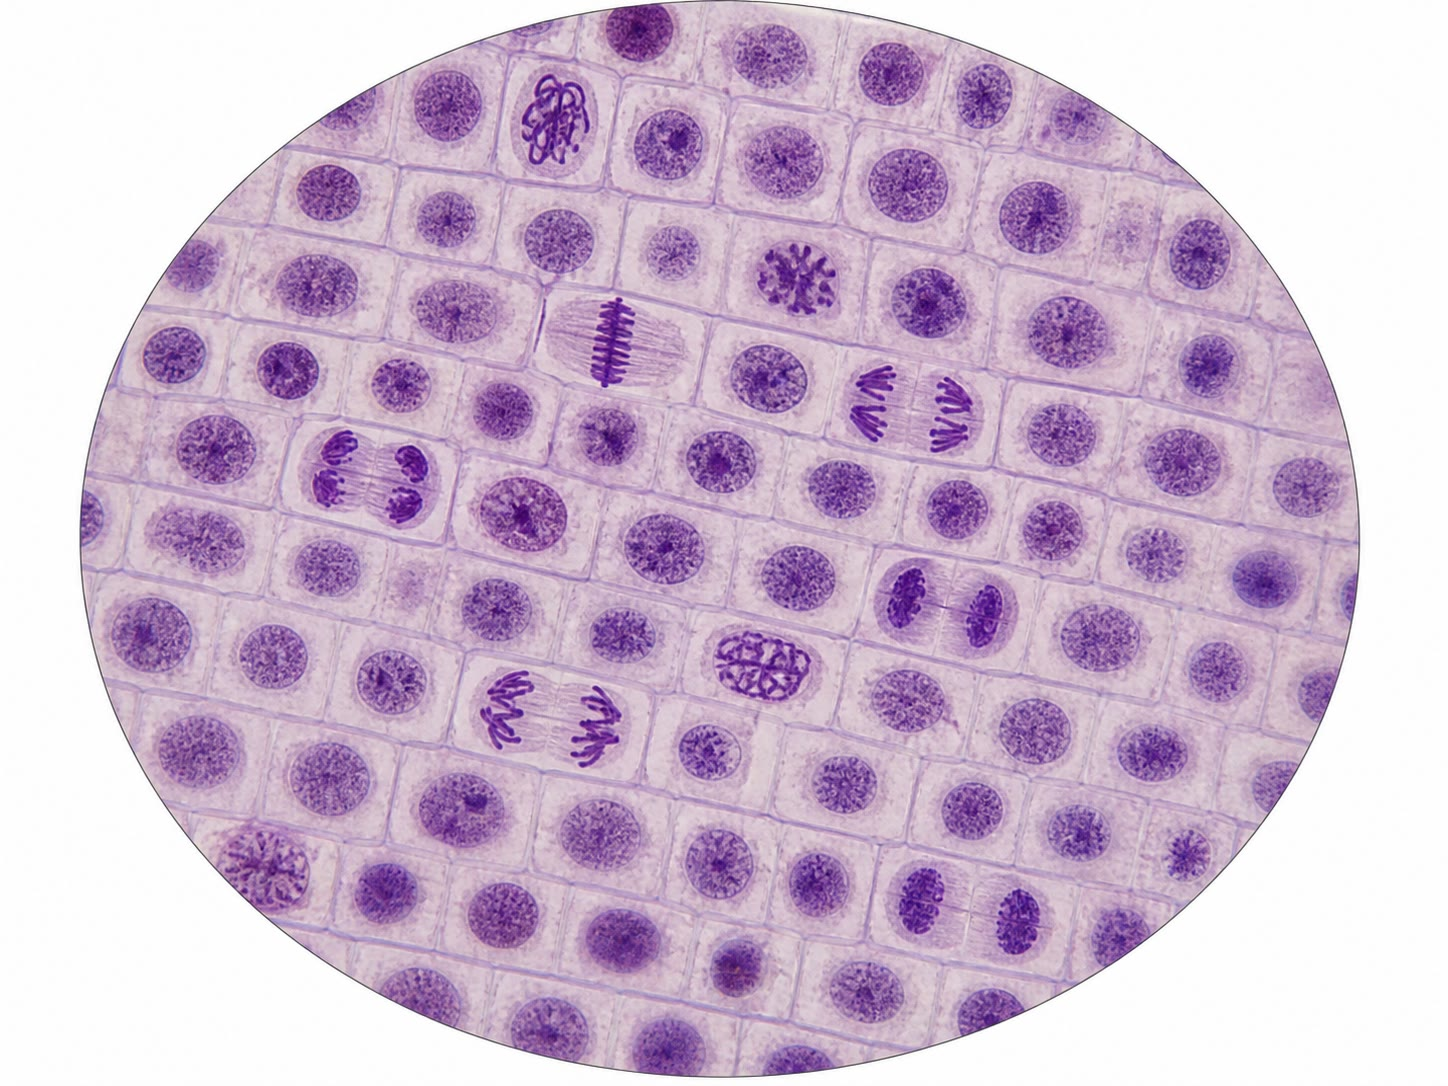
\includegraphics[width=0.58\linewidth]{images/book2/ai/g11-mitosis-root-tip.jpg}

{\small प्रकाश सूक्ष्मदर्शी के नीचे प्याज़ की जड़ के सिरे का कुचला हुआ
नमूना। अधिकांश \omterm{def:g10:cells-common-unit:cell}{कोशिकाएँ} अंतरावस्था में हैं; और कुछ \omterm{def:g11:cell-cycle-mitosis:cycle}{समसूत्री विभाजन} की
अलग-अलग अवस्थाओं में सिकुड़े हुए \omterm{def:g11:cell-cycle-mitosis:chromosome}{गुणसूत्र} दिखाती हैं। हर अवस्था में
\omterm{def:g10:cells-common-unit:cell}{कोशिकाओं} का अनुपात गिनने से पता चलता है कि हर अवस्था कितनी देर चलती है।}
\end{omfigure}

\begin{example}[जड़ के सिरे में गिनती]\label{ex:g11:cell-cycle-mitosis:count}
जड़ के सिरे में गिनी गई 600 \omterm{def:g10:cells-common-unit:cell}{कोशिकाओं} में से 540 अंतरावस्था में हैं और 60
\omterm{def:g11:cell-cycle-mitosis:cycle}{समसूत्री विभाजन} में: यानी 10\% का \emph{समसूत्री सूचकांक}। यदि चक्र 20
घंटे चले, तो \omterm{def:g11:cell-cycle-mitosis:cycle}{समसूत्री विभाजन} लगभग $0.10 \times 20 = \qty{2}{h}$ चलता है;
और यदि विभाजित होती उन 60 \omterm{def:g10:cells-common-unit:cell}{कोशिकाओं} में से 36 पूर्वावस्था में हों, तो
पूर्वावस्था उन दो घंटों का $36/60$ भाग लेती है, यानी क़रीब 72 मिनट, जबकि
पश्चावस्था, जो केवल 4 \omterm{def:g10:cells-common-unit:cell}{कोशिकाओं} में दिखी, लगभग 8 मिनट। सबसे विरली अवस्था
ही सबसे तेज़ है।
\end{example}

\begin{method}[गुणसूत्र और क्रोमैटिड गिनना]\label{met:g11:cell-cycle-mitosis:counting}
$2n$ \omterm{def:g10:universal-dna:information}{गुणसूत्रों} वाली किसी \omterm{def:g10:biodiversity-scales:species}{जाति} के लिए:
\begin{enumerate}
  \item $\mathrm{G_1}$ में: $2n$ \omterm{def:g11:cell-cycle-mitosis:chromosome}{गुणसूत्र}, हर एक में एक \omterm{def:g11:cell-cycle-mitosis:chromosome}{क्रोमैटिड}, \omterm{def:g10:universal-dna:information}{DNA}
        $q$;
  \item S के बाद, $\mathrm{G_2}$, पूर्वावस्था और मध्यावस्था भर: $2n$
        \omterm{def:g11:cell-cycle-mitosis:chromosome}{गुणसूत्र}, हर एक में दो \omterm{def:g11:cell-cycle-mitosis:chromosome}{क्रोमैटिड} ($4n$ \omterm{def:g11:cell-cycle-mitosis:chromosome}{क्रोमैटिड}), \omterm{def:g10:universal-dna:information}{DNA} $2q$;
  \item पश्चावस्था से: \omterm{def:g10:cells-common-unit:cell}{कोशिका} में एक-एक \omterm{def:g11:cell-cycle-mitosis:chromosome}{क्रोमैटिड} वाले $4n$ \omterm{def:g11:cell-cycle-mitosis:chromosome}{गुणसूत्र}, और
        हर ध्रुव की ओर बढ़ते $2n$;
  \item हर पुत्री \omterm{def:g10:cells-common-unit:cell}{कोशिका} में: $2n$ \omterm{def:g11:cell-cycle-mitosis:chromosome}{गुणसूत्र}, हर एक में एक \omterm{def:g11:cell-cycle-mitosis:chromosome}{क्रोमैटिड}, \omterm{def:g10:universal-dna:information}{DNA}
        $q$।
\end{enumerate}
कोई \omterm{def:g11:cell-cycle-mitosis:chromosome}{क्रोमैटिड} उसी क्षण \omterm{def:g11:cell-cycle-mitosis:chromosome}{गुणसूत्र} बन जाता है जब उसका \omterm{def:g11:cell-cycle-mitosis:chromosome}{सेंट्रोमियर} बँटता है।
\end{method}

\begin{example}[मानव के अंक]\label{ex:g11:cell-cycle-mitosis:human}
मध्यावस्था में मानव \omterm{def:g10:cells-common-unit:cell}{कोशिका} 46 \omterm{def:g11:cell-cycle-mitosis:chromosome}{गुणसूत्र} और 92 \omterm{def:g11:cell-cycle-mitosis:chromosome}{क्रोमैटिड} थामे रहती है;
पश्चावस्था में 92 \omterm{def:g11:cell-cycle-mitosis:chromosome}{गुणसूत्र}, जिनमें से 46 हर ध्रुव की ओर बढ़ते हैं; और हर
पुत्री में एक-एक \omterm{def:g11:cell-cycle-mitosis:chromosome}{क्रोमैटिड} वाले 46 \omterm{def:g11:cell-cycle-mitosis:chromosome}{गुणसूत्र}, जिनमें ठीक उतना ही \omterm{def:g10:universal-dna:information}{DNA} है
जितना माता के पास उसके चक्र के आरंभ में था।
\end{example}

\section{समसूत्री विभाजन किस काम का है}

\begin{proposition}[एकरूपता और उसके उपयोग]\label{prop:g11:cell-cycle-mitosis:conformity}
चूँकि प्रतिकृतिकरण भरोसेमंद है और \omterm{def:g11:cell-cycle-mitosis:cycle}{समसूत्री विभाजन} \omterm{def:g11:cell-cycle-mitosis:chromosome}{क्रोमैटिडों} को ठीक-ठीक
बाँटता है, इसलिए किसी बहुकोशिकीय शरीर की हर \omterm{def:g10:cells-common-unit:cell}{कोशिका} वही \omterm{def:g10:universal-dna:information}{आनुवंशिक जानकारी}
ढोती है जो उस निषेचित अंडाणु में थी जिससे वह उतरी है। \omterm{def:g11:cell-cycle-mitosis:cycle}{समसूत्री विभाजन}
वृद्धि की क्रियाविधि है (भ्रूण, जड़ का सिरा), नवीकरण की (त्वचा, आँत की
परत, रक्त: अकेली अस्थि मज्जा हर दिन क़रीब $\num{2e11}$ \omterm{def:g10:cells-common-unit:cell}{कोशिकाएँ} बनाती है)
और मरम्मत की (घाव भरना); और एककोशिकीय सुकेंद्रकियों में वही ख़ुद जनन है।
उसका नियंत्रण --- चक्र में घुसने का फ़ैसला, तथा S से पहले और पश्चावस्था
से पहले की जाँचें --- \cref{ch:g11:cancer} का विषय है।
\end{proposition}
\admitted

\begin{remark}[हर चीज़ विभाजित नहीं होती]\label{rem:g11:cell-cycle-mitosis:notall}
अधिकांश न्यूरॉन और हृदय की पेशी \omterm{def:g10:cells-common-unit:cell}{कोशिकाएँ} बचपन में ही चक्र छोड़ देती हैं
और उसमें कभी नहीं लौटतीं: उन्हें पहुँचा नुक़सान विभाजन से नहीं भरता, और
इसीलिए मेरुरज्जु की चोट या दिल का दौरा टिकी हुई हानि छोड़ जाता है। यकृत
की \omterm{def:g10:cells-common-unit:cell}{कोशिकाएँ} महीनों तक $\mathrm{G_1}$ में विश्राम करती हैं, पर यकृत का एक
हिस्सा हटा देने पर चक्र में लौट आती हैं और हफ़्तों में अंग दोबारा उगा देती
हैं। कौन-सी \omterm{def:g10:cells-common-unit:cell}{कोशिकाएँ} विभाजित हो सकती हैं और कब, यह शरीर के सबसे कड़े
नियंत्रणों में से एक है।
\end{remark}

\section{अभ्यास}

\begin{exercise}[$\star$]\label{exo:g11:cell-cycle-mitosis:1}
\omterm{def:g11:cell-cycle-mitosis:cycle}{कोशिका चक्र} की चारों प्रावस्थाओं के नाम लिखिए और हर एक में क्या होता है
यह भी बताइए।
\end{exercise}

\begin{exercise}[$\star$]\label{exo:g11:cell-cycle-mitosis:2}
\omterm{def:g11:cell-cycle-mitosis:chromosome}{क्रोमैटिड} और \omterm{def:g11:cell-cycle-mitosis:chromosome}{सेंट्रोमियर} की परिभाषा दीजिए। किसी \omterm{def:g11:cell-cycle-mitosis:chromosome}{गुणसूत्र} में दो \omterm{def:g11:cell-cycle-mitosis:chromosome}{क्रोमैटिड}
कब होते हैं?
\end{exercise}

\begin{exercise}[$\star$]\label{exo:g11:cell-cycle-mitosis:3}
\omterm{def:g11:cell-cycle-mitosis:cycle}{समसूत्री विभाजन} की चारों अवस्थाएँ एक-एक मुख्य घटना के साथ गिनाइए।
\end{exercise}

\begin{exercise}[$\star$]\label{exo:g11:cell-cycle-mitosis:4}
किसी \omterm{def:g10:cells-common-unit:organelle}{केंद्रक} में \omterm{def:g10:universal-dna:information}{DNA} की मात्रा $1.5q$ है। \omterm{def:g10:cells-common-unit:cell}{कोशिका} किस प्रावस्था में है?
\end{exercise}

\begin{exercise}[$\star$]\label{exo:g11:cell-cycle-mitosis:5}
$\mathrm{G_2}$ में किसी मानव \omterm{def:g10:cells-common-unit:cell}{कोशिका} में कितने \omterm{def:g11:cell-cycle-mitosis:chromosome}{गुणसूत्र} और कितने \omterm{def:g11:cell-cycle-mitosis:chromosome}{क्रोमैटिड}
होते हैं?
\end{exercise}

\begin{exercise}[$\star\star$]\label{exo:g11:cell-cycle-mitosis:6}
\omterm{def:g10:universal-dna:information}{DNA} की मात्रा वाले चित्र से हर प्रावस्था की अवधि बताइए, और यह भी कि $2q$
वाली \omterm{def:g10:cells-common-unit:cell}{कोशिका} किन प्रावस्थाओं में मिल सकती है।
\end{exercise}

\begin{exercise}[$\star\star$]\label{exo:g11:cell-cycle-mitosis:7}
किसी चूहे में $2n = 40$ है। मध्यावस्था में, पश्चावस्था में (पूरी \omterm{def:g10:cells-common-unit:cell}{कोशिका}),
और किसी पुत्री \omterm{def:g10:cells-common-unit:cell}{कोशिका} में \omterm{def:g10:universal-dna:information}{गुणसूत्रों} तथा \omterm{def:g11:cell-cycle-mitosis:chromosome}{क्रोमैटिडों} की संख्या बताइए।
\end{exercise}

\begin{exercise}[$\star\star$]\label{exo:g11:cell-cycle-mitosis:8}
जड़ के किसी सिरे में 800 \omterm{def:g10:cells-common-unit:cell}{कोशिकाएँ} गिनी जाती हैं: 720 अंतरावस्था में, 48
पूर्वावस्था में, 16 मध्यावस्था में, 6 पश्चावस्था में, 10 अंत्यावस्था में।
समसूत्री सूचकांक और, 24 घंटे के चक्र के लिए, हर अवस्था की अवधि निकालिए।
\end{exercise}

\begin{exercise}[$\star\star$]\label{exo:g11:cell-cycle-mitosis:9}
कोल्चिसीन, जो पतझड़ के क्रोकस से निकाली गई दवा है, तर्कु को बनने से रोक
देती है। उससे उपचारित किसी विभाजित होती \omterm{def:g10:cells-common-unit:cell}{कोशिका} का क्या होगा, इसका अनुमान
लगाइए, और यह भी कि जीवविज्ञानी उसे \omterm{def:g11:cell-cycle-mitosis:chromosome}{गुणसूत्र-चित्र} बनाने के लिए क्यों
इस्तेमाल करते हैं।
\end{exercise}

\begin{exercise}[$\star\star$]\label{exo:g11:cell-cycle-mitosis:10}
समझाइए कि \omterm{def:g10:universal-dna:information}{गुणसूत्रों} को हिलाने से पहले उनका सिकुड़ना क्यों ज़रूरी है, और
बाद में वे दोबारा क्यों खुल जाते हैं।
\end{exercise}

\begin{exercise}[$\star\star$]\label{exo:g11:cell-cycle-mitosis:11}
कोई निषेचित अंडाणु पहले दिनों में हर 12 घंटे में विभाजित होता है। 5 दिन
बाद कितनी \omterm{def:g10:cells-common-unit:cell}{कोशिकाएँ} होंगी? क्या हर विभाजन को पूरा $\mathrm{G_1}$ चाहिए
होगा?
\end{exercise}

\begin{exercise}[$\star\star\star$]\label{exo:g11:cell-cycle-mitosis:12}
पश्चावस्था में किसी एक \omterm{def:g11:cell-cycle-mitosis:chromosome}{गुणसूत्र} के दोनों \omterm{def:g11:cell-cycle-mitosis:chromosome}{क्रोमैटिड} अलग होने में चूक जाते
हैं और दोनों एक ही ध्रुव पर चले जाते हैं। दोनों पुत्री \omterm{def:g10:cells-common-unit:cell}{कोशिकाओं} का वर्णन
कीजिए (\omterm{def:g11:cell-cycle-mitosis:chromosome}{गुणसूत्र} संख्या, \omterm{def:g10:universal-dna:information}{DNA}) और समझाइए कि किसी शरीर \omterm{def:g10:cells-common-unit:cell}{कोशिका} में ऐसी ग़लती
आमतौर पर बेअसर क्यों रहती है, पर कुछ हालों में गंभीर क्यों हो जाती है।
\end{exercise}

\begin{exercise}[$\star\star\star$]\label{exo:g11:cell-cycle-mitosis:13}
अस्थि मज्जा हर दिन $\num{2e11}$ रक्त \omterm{def:g10:cells-common-unit:cell}{कोशिकाएँ} बनाती है। यदि मज्जा की कोई
पूर्वगामी \omterm{def:g10:cells-common-unit:cell}{कोशिका} 24 घंटे में चक्र पूरा करती हो, तो आँकिए कि किसी भी क्षण
कितनी पूर्वगामी \omterm{def:g10:cells-common-unit:cell}{कोशिकाएँ} विभाजित हो रही हैं, और टिप्पणी कीजिए कि \omterm{def:g11:cell-cycle-mitosis:cycle}{समसूत्री
विभाजन} रोकने वाली कोई दवा हफ़्ते भर में रक्त का क्या हाल करती।
\end{exercise}

\begin{exercise}[$\star\star\star$]\label{exo:g11:cell-cycle-mitosis:14}
समझाइए कि \omterm{def:g11:cell-cycle-mitosis:chromosome}{गुणसूत्र-चित्र} अंतरावस्था या पश्चावस्था के बजाय मध्यावस्था में
रोकी गई \omterm{def:g10:cells-common-unit:cell}{कोशिकाओं} से क्यों बनाया जाता है।
\end{exercise}

\begin{exercise}[$\star\star\star$]\label{exo:g11:cell-cycle-mitosis:15}
किसी यकृत का दो-तिहाई हटा दिया जाता है; और तीन हफ़्तों में वह दोबारा उग
आता है। \omterm{def:g11:cell-cycle-mitosis:cycle}{कोशिका चक्र} की मदद से बताइए कि उसकी \omterm{def:g10:cells-common-unit:cell}{कोशिकाओं} ने क्या किया, और यह
भी कि दिन 0 के मुक़ाबले दिन 3 पर यकृत \omterm{def:g10:cells-common-unit:cell}{कोशिकाओं} की DNA-मात्रा कैसी दिखती।
\end{exercise}

\section{समस्या: जड़ के सिरे की समय-सारणी}

\begin{problem}[{सप्ताहांत समस्या --- जड़ का एक सिरा कोशिका-दर-कोशिका
गिना गया: चक्र की हर अवस्था की लंबाई, हर क्षण का DNA, कोई जड़ दिन भर में
कितनी कोशिकाएँ बनाती है, और पश्चावस्था के वे आठ मिनट}]
\label{pb:g11:cell-cycle-mitosis:1}
एक कक्षा लहसुन की जड़ का सिरा ($2n = 16$) कुचलकर और रँगकर वृद्धि क्षेत्र
की 1000 \omterm{def:g10:cells-common-unit:cell}{कोशिकाएँ} गिनती है: 900 अंतरावस्था में, 60 पूर्वावस्था में, 18
मध्यावस्था में, 8 पश्चावस्था में, 14 अंत्यावस्था में। स्वतंत्र मापें इन
\omterm{def:g10:cells-common-unit:cell}{कोशिकाओं} का चक्र 20 घंटे बताती हैं। वृद्धि क्षेत्र में 20\,000 \omterm{def:g10:cells-common-unit:cell}{कोशिकाएँ}
मान लीजिए।

\medskip
\noindent\textbf{भाग I --- समसूत्री सूचकांक।}
\begin{enumerate}
  \item उस ऊतक का समसूत्री सूचकांक निकालिए।
  \item यह मानते हुए कि किसी अवस्था में \omterm{def:g10:cells-common-unit:cell}{कोशिकाओं} का अंश उस अवस्था में
        बीते चक्र के अंश के बराबर है, \omterm{def:g11:cell-cycle-mitosis:cycle}{समसूत्री विभाजन} की अवधि निकालिए।
  \item चारों अवस्थाओं में से हर एक की अवधि निकालिए।
  \item सबसे छोटी अवस्था कौन-सी है? सुझाइए कि वह इतनी तेज़ क्यों हो सकती
        है।
  \item यह विधि बहुत-सी \omterm{def:g10:cells-common-unit:cell}{कोशिकाएँ} गिनने की माँग क्यों करती है, और वे केवल
        वृद्धि क्षेत्र से ही क्यों आनी चाहिए?
\end{enumerate}

\medskip
\noindent\textbf{भाग II --- \omterm{def:g11:cell-cycle-mitosis:chromosome}{गुणसूत्र} और \omterm{def:g10:universal-dna:information}{DNA}।}
\begin{enumerate}[resume]
  \item मध्यावस्था में लहसुन की \omterm{def:g10:cells-common-unit:cell}{कोशिका} कितने \omterm{def:g11:cell-cycle-mitosis:chromosome}{गुणसूत्र} और कितने \omterm{def:g11:cell-cycle-mitosis:chromosome}{क्रोमैटिड}
        थामे रहती है?
  \item पश्चावस्था वाली \omterm{def:g10:cells-common-unit:cell}{कोशिका} में कितने \omterm{def:g11:cell-cycle-mitosis:chromosome}{गुणसूत्र} चल रहे होते हैं, और हर
        ध्रुव तक कितने पहुँचते हैं?
  \item पुत्री \omterm{def:g10:cells-common-unit:cell}{कोशिका} के \omterm{def:g10:universal-dna:information}{DNA} को $q$ कहते हुए पूर्वावस्था वाली, पश्चावस्था
        वाली (पूरी \omterm{def:g10:cells-common-unit:cell}{कोशिका}) और अंत्यावस्था वाली (हर \omterm{def:g10:cells-common-unit:organelle}{केंद्रक}) \omterm{def:g10:cells-common-unit:cell}{कोशिका} की
        DNA-मात्रा बताइए।
  \item यदि $\mathrm{G_1}$, S और $\mathrm{G_2}$ क्रमशः 8, 7 और 4 घंटे
        लेते हों, तो अंतरावस्था वाली उन 900 \omterm{def:g10:cells-common-unit:cell}{कोशिकाओं} में से मोटे तौर पर
        कितनी S में हैं?
  \item किसी विद्यार्थी को ऐसी \omterm{def:g10:cells-common-unit:cell}{कोशिका} मिलती है जिसमें एक-एक \omterm{def:g11:cell-cycle-mitosis:chromosome}{क्रोमैटिड}
        वाले 32 \omterm{def:g11:cell-cycle-mitosis:chromosome}{गुणसूत्र} \omterm{def:g10:cells-common-unit:cell}{कोशिकाद्रव्य} भर फैले हैं। वह कौन-सी अवस्था है,
        और अभी-अभी क्या हुआ है?
\end{enumerate}

\medskip
\noindent\textbf{भाग III --- जड़ का उत्पादन।}
\begin{enumerate}[resume]
  \item यदि वृद्धि क्षेत्र की हर \omterm{def:g10:cells-common-unit:cell}{कोशिका} 20 घंटे में चक्र पूरा करती हो, तो
        वह क्षेत्र प्रति घंटा कितनी नई \omterm{def:g10:cells-common-unit:cell}{कोशिकाएँ} बनाता है?
  \item वृद्धि क्षेत्र से बाहर निकलते ही हर नई \omterm{def:g10:cells-common-unit:cell}{कोशिका} लंबी होकर लगभग
        \qty{100}{\micro m} की हो जाती है। एक \omterm{def:g10:cells-common-unit:cell}{कोशिका} चौड़ी किसी क़तार
        में जड़ प्रति दिन कितनी लंबी होगी? देखी गई प्रति दिन \qty{1}{mm}
        से तुलना कीजिए और फ़र्क़ समझाइए।
  \item हर पुत्री \omterm{def:g10:cells-common-unit:cell}{कोशिका} को $2n = 16$ \omterm{def:g10:universal-dna:information}{गुणसूत्रों} की, यानी कुल मिलाकर
        क़रीब $\num{1.6e10}$ क्षारक-जोड़ों की, नक़ल करनी होती है। प्रति
        सेकंड 50 \omterm{def:g10:universal-dna:nucleotide}{न्यूक्लियोटाइड} वाले द्विशाखों के साथ S के 7 घंटों में
        काम पूरा करने के लिए कितने प्रारंभ स्थल चाहिए?
  \item जड़ को दिन भर के लिए ठंड में (\qty{4}{\celsius}) रखा जाता है।
        गिनतियों में बदलाव का, और यदि ठंड सारी प्रावस्थाओं को बराबर धीमा
        करे तो समसूत्री सूचकांक में बदलाव का, अनुमान लगाइए।
  \item कोई शाकनाशी \omterm{prop:g11:dna-replication:forks}{DNA पॉलिमरेज़} को रोक देता है। दिन भर बाद कुचले हुए
        नमूने में कौन-सी अवस्थाएँ अब भी दिखतीं और कौन-सी ग़ायब हो चुकी
        होतीं? समझाइए।
\end{enumerate}

\medskip
\noindent\textbf{भाग IV --- गिनतियों का फ़ैसला।}
\begin{enumerate}[resume]
  \item दूसरी कक्षा उसी ऊतक को गिनती है और 1000 \omterm{def:g10:cells-common-unit:cell}{कोशिकाओं} में 4
        पश्चावस्थाएँ पाती है। वे कौन-सी अवधि निकालेंगे? मुट्ठी भर
        \omterm{def:g10:cells-common-unit:cell}{कोशिकाओं} में दिखने वाली अवस्था के लिए यह असहमति चौंकाने वाली है?
  \item दोनों कक्षाओं को मिलाकर (2000 \omterm{def:g10:cells-common-unit:cell}{कोशिकाएँ}, 12 पश्चावस्थाएँ)
        पश्चावस्था की अवधि दोबारा निकालिए।
  \item संवर्धन में उगाई मानव \omterm{def:g10:cells-common-unit:cell}{कोशिकाओं} का समसूत्री सूचकांक 4\% है और चक्र
        24 घंटे का। उनके \omterm{def:g11:cell-cycle-mitosis:cycle}{समसूत्री विभाजन} की अवधि की लहसुन वाली अवधि से
        तुलना कीजिए।
  \item समझाइए कि किसी अर्बुद का समसूत्री सूचकांक उस ऊतक से, जिससे वह
        उठा है, अक्सर कई गुना अधिक क्यों होता है, और तर्कु पर असर करने
        वाली किसी दवा के लिए उसका क्या मतलब है।
  \item परिणाम लिखिए: लहसुन की जड़ की \omterm{def:g10:cells-common-unit:cell}{कोशिका} के चक्र की अवस्था-दर-अवस्था
        समय-सारणी, और वह अवस्था जिसके आठ मिनट यह तय करते हैं कि हर पुत्री
        को सोलह \omterm{def:g11:cell-cycle-mitosis:chromosome}{गुणसूत्र} मिलें।
\end{enumerate}
\end{problem}
